\documentclass[letter]{article}

\usepackage{ijcai15}
\usepackage{times}

\usepackage{eurosym}
\usepackage{hyperref}		% clickable references

\usepackage{apacite}            % APA style citations
\usepackage{apacdoc}
\usepackage{mdframed}

\usepackage{amsmath,amssymb}	% math structures and symbols
\usepackage{graphicx}		% including of graphics files in various formats
\usepackage{amsfonts}
\usepackage{dialogue}
\usepackage{placeins}
\usepackage{tikz}
\usetikzlibrary{positioning,backgrounds,fit,arrows,shapes,shadows}
\usetikzlibrary{shapes.multipart}
\usepackage{wrapfig}
\usepackage{enumitem}
\usepackage{framed}

% \hypersetup{hidelinks}

\usepackage[xspace,mla]{ellipsis}

\definecolor{myyellow}{RGB}{242,226,149}
\definecolor{mygreen}{RGB}{144,238,144}
\definecolor{mypink}{RGB}{255,182,193}
\definecolor{myorange}{RGB}{255,165,0}
\definecolor{myblue}{RGB}{0,204,204}

\usepackage{xparse}
\NewDocumentCommand\StickyNote{O{4cm}mmO{4cm}}{%
\begin{tikzpicture}
\node[
drop shadow={
  shadow xshift=2pt,
  shadow yshift=-4pt
},
inner xsep=7pt,
fill=#2,
xslant=-0.05,
yslant=0.05,
inner ysep=10pt
] {\parbox[t][#1][c]{#4}{#3}};
\end{tikzpicture}%
}

\urldef{\mailsa}\path|{j.corneli,s.colton}@gold.ac.uk|
\urldef{\mailsb}\path|a.pease@dundee.co.uk|

\newcommand{\Fw}{{\sf FloWr}}
\newcommand{\dec}[1]{\raisebox{.2ex}{$\star$}#1\raisebox{.2ex}{$\star$}}

\newcommand{\keywords}[1]{\par\addvspace\baselineskip
\noindent\keywordname\enspace\ignorespaces#1}

\begin{document}

% TITLE INFORMATION
\title{Implementing feedback in creative systems}

\author{Joseph Corneli\textsuperscript{1} and Anna Jordanous\textsuperscript{2}\\
\textsuperscript{1} Department of Computing, Goldsmiths College, University of London\\
\textsuperscript{2} School of Computing, University of Kent}

\date{today}

\maketitle

\begin{abstract} 
% First attempt
%% Various social strategies, ranging from Writers Workshops to open
%% source software, pair programming, and design charettes have been
%% developed to exploit emergent effects and to develop new shared
%% language.  We investigate the feasibility of using designs of this
%% sort in multi-agent systems that learn by sharing and discussing
%% partial understandings.  Building on earlier theoretical work, we
%% describe concrete implementation plans and some preliminary results.
\end{abstract}

% END OF COMMENTED OUT PART


\section{Implementation plans and preliminary results}\label{sec:implementation}

Add $\approx$1 page...

\section{Ideas}

Some images from \emph{Aesthetic Complexity: Practice and Perception in Art \& Design}\footnote{\url{https://aestheticcomplexity.wordpress.com/research/phd/}}

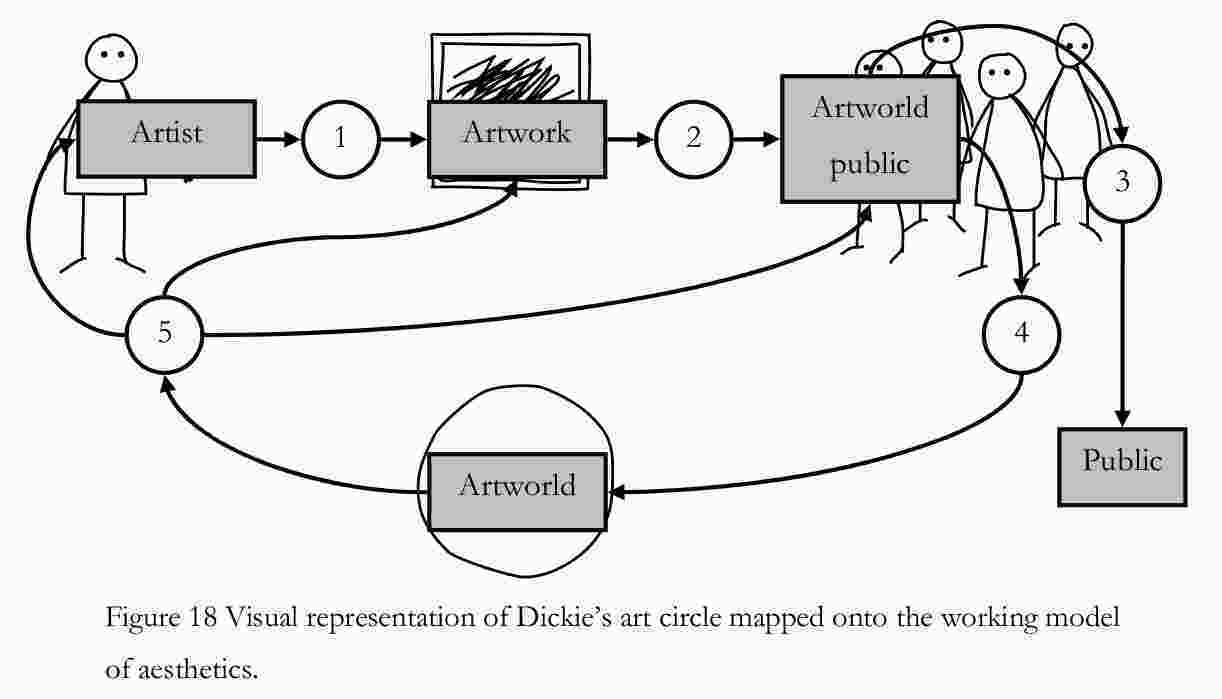
\includegraphics[width=\columnwidth]{./figures/artworld.jpg}

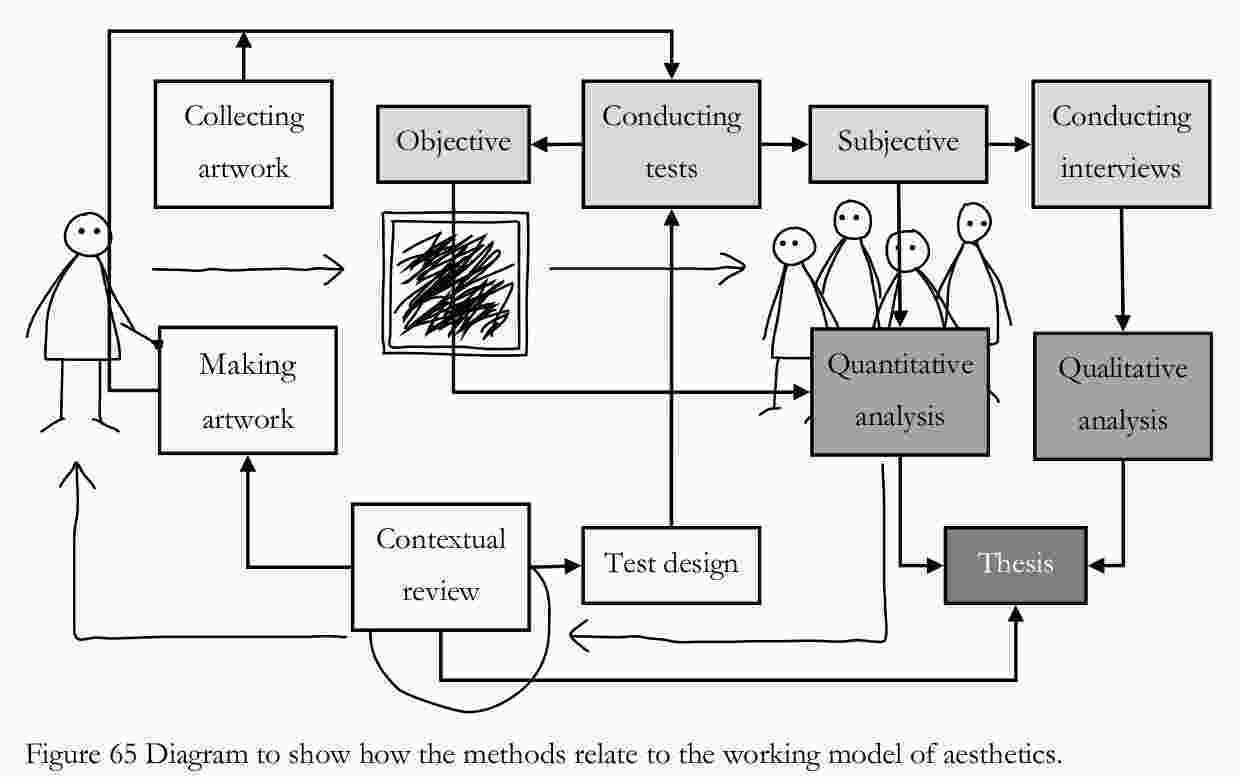
\includegraphics[width=\columnwidth]{./figures/aesthetic-research.jpg}

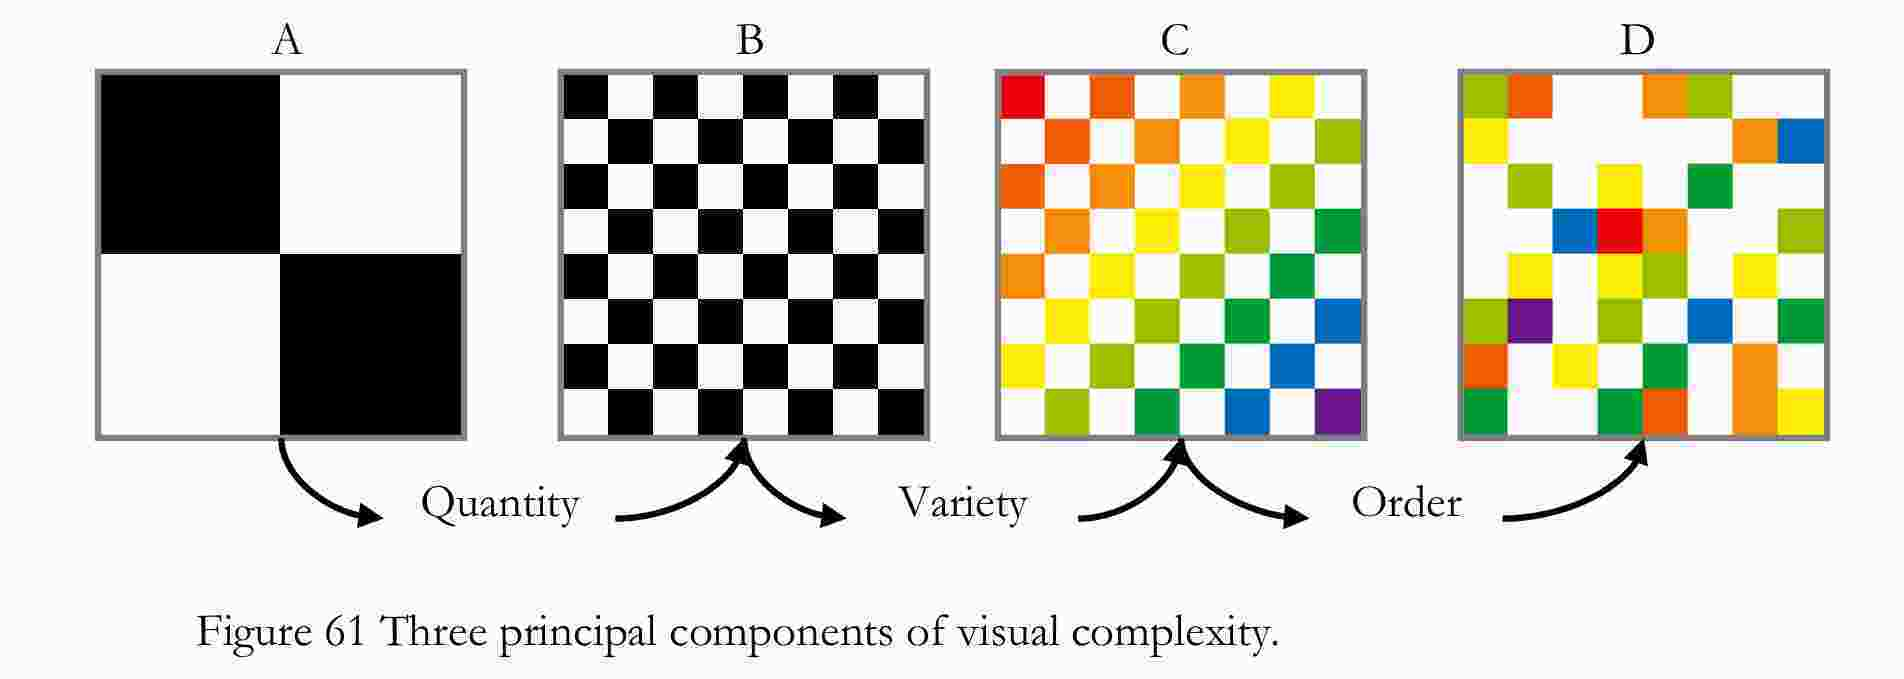
\includegraphics[width=\columnwidth]{./figures/quantity-variety-order.jpg}


%%COmment out 
%\bibliographystyle{apacite}
%\bibliography{./biblio}

%\end{document}

%% To the extent possible, exchanges of dialogue such as the example given in Section \ref{sec:writers-workshop} in the process language should be a
%% matter of dynamics rather than representation: this is another way to
%% say that ``triggers'' should be independent of their ``results.''
%% Someone saying something in the workshop does not cause the
%% participant to act, but rather, to think.
%% In order to facilitate this sort of interaction, it would be necessary
%% for systems to implement a basic protocol related to
%% %%
%% {\tt presentation}, {\tt listening}, {\tt
%%   feedback}, {\tt questions}, and {\tt
%%   reflections}.
%% %%

%% \begin{description}
%% \item[Presentation:] definition ***
%% \item[Listening:] definition ***
%% \item[Feedback:] definition ***
%% \item[Questions:] definition ***
%% \item[Reflections:] definition ***
%% \end{description}

% First attempt
%% Various social strategies, ranging from Writers Workshops to open
%% source software, pair programming, and design charettes have been
%% developed to exploit emergent effects and to develop new shared
%% language.  We investigate the feasibility of using designs of this
%% sort in multi-agent systems that learn by sharing and discussing
%% partial understandings.  Building on earlier theoretical work, we
%% describe concrete implementation plans and some preliminary results.
%%
%%
%%
% \item[] Research question: \emph{How do we implement feedback in
%  creative systems?}

There are similarities between the
Writers Workshops and classical practices of group composition
\cite{jin1975art} and dialectic \cite{dialectique}, and the workshop
may be considered an artistic or creative space in its own right.


\begin{mdframed}
{\large Some things we can (potentially) feed into the survey above,
  or delete if they are not useful.}

\begin{enumerate}[start=2]
\item \textbf{Here we refine the idea and turn it into a general model
  that for incorporating feedback within computational models of the
  creative process.}
\item[] Intuitive examples of application areas
\begin{enumerate}
\item learning/training
%% Supervised learning,
%% Reinforcement learning (Temporal Difference Learning)
%% Evolution
\item guidance/control
\end{enumerate}
\item[] What can feedback be about in general terms? \dec{Survey}
\begin{enumerate}
\item Progress relative to explicit or adduced \emph{exploration}
  (knowledge and accuracy) or \emph{exploitation} (directional,
  task-based) goals.
\item \emph{Quantity}, \emph{Variety}, and \emph{Order} of produced
  objects or behaviours
\item New relationships among produced objects and behaviours drawing
  on a common field of reference
\end{enumerate}
\item[] How can feedback be understood and used? \dec{Survey}
\begin{enumerate}
\item Update knowledge base with new facts (accept statements,
  possibly with provenance)
\item Note similarity to \emph{iterative development}
\item Reflection: describe relationships between produced objects and
  behaviours and feedback
\item Reflection: Higher-order patterns e.g.~new patterns that
  describe the identified exceptions
\end{enumerate}
\end{enumerate}

\begin{enumerate}[start=4]
\item \textbf{Discussion of how this would work more generally in
  computational creativity and perhaps in AI more generally with an
  eye toward producing effects like ``serendipity'' and
  ``emergence.''}
\begin{enumerate}
\item ``Artificial and natural intelligence are both search'' -- you learn a few concepts the hard way and then use them to understand things you only have one shot at (Metaphors we live by).  Neo-diffusionist hypothesis: culture is like any other feature, if it helps you, you're more likely to keep it.  (Kashima).  Deacon's ``Theory of semantics''.  Human semantics can be replicated by statistical learning on large corpora.  Finch 1993, Bilovich and Bryson 2008.  The 75 second most frequent words give a good match to human semantics.  McDonald and Lowe, check the cosines.  Implicit University of Bath, Macfarlane.  Bryson 2008, Theory of Semantics.  ``What are the things that need to be preserved and what are the things that we can mutate?''  Primates not only remember how people treat themselves, they also remember how they treat each other (Second Order representation).  Evolvability is something that AI reseachers should be getting their hands on.  Dual replicators: culture and biology both evolve.  Within the genome, there are hierarchical representations and genes to flag ``zones of innovation'' (Richard Watson, machine learning, genetics, and evolvability)  Cross-over lets you stay close to the fitness peak (Yifei Wang).  \v{C}a\v{c}e and Bryson 2007, agent based modelling of communication costs, in Emergence and Evolution of Linguistic Communication.  ``What is transmitted is the replicator, but the unit of selection is the vehicle/interactor.''  Simpson's paradox.  Daniel Taylor, Evolution of the Social Contract -- everything is semi-private, disseration.  Lots of ways to create modular systems.  Jekaterina Novikova, transparently synthetic emotions for collaboration.  Swen Gaudl, learning from observation of human players and then coming up with better versions of the game using genetic programming.  London Futurists.  Human language and our values come out of our experiences and our \emph{sociality}.  E.g. punishing someone for being antisocial is contributing to your own good.  ``Chimps are moral patients.''
\begin{itemize}
\item (Clark 2013) quotes Ashby.  Homeostatics\ldots Stuff from Anil's talk.
  Wiener 1964 cites Ashby.  Conant and Ashby: ``Every good regulator
  of a system must be a model of that system.''  This leads to the
  ``free energy principle.''  Keep the organism within states in which
  it will receive the kinds of input it expects. 
\item A very intuitive point: customer feedback is a big thing, and
  increasingly present in online commerce and the social web (think
  e.g.~of Yelp).  The particular challenge here is to have the
  resources in order to effectively respond to the feedback.
\item Another philosophical point (maybe we can bring it in earlier)
  is that in the Writers Workshop model, feedback is somehow an
  economic ``externality.''  That is, the author gets the feedback
  ``for free.''  Other applications of the idea would be similar.
  This kicks off a number of related questions.
\item The first question is about ``how integrated'' the systems
  should be.  Are we willing to call an action taken by the system
  itself `feedback'?  Probably not: for that appelation we would
  require interaction with the world, causally determined but in some
  way stochastic effects.
\item This is related to Bergson's discussion of \emph{reflex} and
  (especially) Coase's discussion of firms.  In a more AI setting,
  this relates to the idea of \emph{sensors} and \emph{effectors}.  In
  dialogue models there are ideas of ``deontic scoreboards''
  (Brandom, Walton).
\item Different traditions in cognitive science: predictive processing
  e.g.~von Helmholtz.  The brain has no direct access.  There are
  uncertain signals about actual things in the world; so the brain
  needs to use inference.  (Clark 2013 BBS) The beholder's share.
  This maps onto ideas of predictive processing in cortical networks.
  Top down convey predictions, bottom up convey prediction errors
  (French 2009 Trends in Cognitive Science).  In the end, there's a
  sensible explanation.  We usually think that bottom up conveys the
  signal; but this outside-in pathway is built on feedback.  How
  strongly should we weight prediction errors versus predictions?
%% Sellars: reliable differential capacities to respond to environmental stimuli
\end{itemize}
\end{enumerate}
\end{enumerate}
\end{mdframed}
\end{document}